\documentclass[11pt]{article}

% ---------- packages ----------
\usepackage[margin=1in]{geometry}
\usepackage{amsmath,amssymb,amsfonts}
\usepackage{bm}
\usepackage{mathtools}
\usepackage{booktabs}
\usepackage{array}
\usepackage{longtable}
\usepackage{enumitem}
\usepackage{xcolor}
\usepackage{tikz}
\usetikzlibrary{positioning,arrows.meta,shapes.geometric,calc,fit,backgrounds,decorations.pathreplacing}
\usepackage{caption}
\usepackage[hidelinks]{hyperref}
\usepackage{parskip}
\usepackage{titlesec}

\titleformat{\section}{\normalfont\Large\bfseries}{\thesection}{0.75em}{}
\titleformat{\subsection}{\normalfont\large\bfseries}{\thesubsection}{0.75em}{}
\captionsetup{font=small,labelfont=bf}

% ---------- colors ----------
\definecolor{phys}{HTML}{2C6E9B}   % physics / layer 1
\definecolor{agent}{HTML}{9B4DA0}  % agent / layer 2
\definecolor{data}{HTML}{C9772B}   % artifacts
\definecolor{ml}{HTML}{2E8B57}     % ML / surrogate
\definecolor{soft}{HTML}{F2F4F7}   % soft background
\definecolor{softblue}{HTML}{E8F0F7}
\definecolor{softpurple}{HTML}{F1E8F2}
\definecolor{softorange}{HTML}{FBEEDD}
\definecolor{softgreen}{HTML}{E6F2EB}

% ---------- tikz styles ----------
\tikzset{
  proc/.style   = {rectangle, rounded corners=2pt, draw=phys!80, fill=softblue,
                   align=center, inner sep=5pt, font=\small, minimum height=8mm},
  mlproc/.style = {rectangle, rounded corners=2pt, draw=ml!80, fill=softgreen,
                   align=center, inner sep=5pt, font=\small, minimum height=8mm},
  agproc/.style = {rectangle, rounded corners=2pt, draw=agent!80, fill=softpurple,
                   align=center, inner sep=5pt, font=\small, minimum height=8mm},
  artifact/.style = {cylinder, shape border rotate=90, aspect=0.25, draw=data!85,
                   fill=softorange, align=center, inner sep=4pt, font=\small\ttfamily,
                   minimum height=9mm, minimum width=20mm},
  decision/.style = {diamond, aspect=1.8, draw=agent!80, fill=softpurple,
                   align=center, inner sep=1pt, font=\small, minimum height=8mm},
  lyr/.style    = {rectangle, rounded corners=3pt, draw=black!25, thick, inner sep=8pt},
  flow/.style   = {-{Stealth[length=2.4mm]}, thick, draw=black!65},
  flowback/.style = {-{Stealth[length=2.4mm]}, thick, draw=agent!70, dashed},
  lbl/.style    = {font=\scriptsize\itshape, text=black!55},
}

% ---------- convenience macros ----------
\newcommand{\bx}{\mathbf{x}}
\newcommand{\bz}{\mathbf{z}}
\newcommand{\by}{\mathbf{y}}
\newcommand{\bc}{\mathbf{c}}
\newcommand{\bw}{\mathbf{w}}
\newcommand{\bK}{\mathbf{K}}
\newcommand{\bV}{\mathbf{V}}
\newcommand{\bU}{\mathbf{U}}
\newcommand{\bI}{\mathbf{I}}
\newcommand{\bSig}{\bm{\Sigma}}
\newcommand{\bPhi}{\bm{\Phi}}
\newcommand{\bphi}{\bm{\phi}}
\newcommand{\bmu}{\bm{\mu}}
\newcommand{\Ffwd}{\mathcal{F}}
\newcommand{\Fhat}{\hat{\mathcal{F}}}
\newcommand{\R}{\mathbb{R}}
\newcommand{\E}{\mathbb{E}}
\newcommand{\GP}{\mathcal{GP}}
\newcommand{\indic}{\mathbb{1}}
\DeclareMathOperator{\Var}{Var}
\DeclareMathOperator{\RMSE}{RMSE}
\DeclareMathOperator*{\argmin}{arg\,min}
\DeclareMathOperator*{\argmax}{arg\,max}
\newcommand{\Lstar}{\Delta^{\!*}}

\title{\textbf{Autotokamak: An Agentic Platform for Learning Fast
Surrogates of the Grad--Shafranov Equilibrium}\\[0.4em]
\large A System Description and Mathematical Reference}
\author{}
\date{}

\begin{document}
\maketitle

\begin{abstract}
\noindent
Autotokamak is a research platform that learns fast machine-learning surrogates for the
Grad--Shafranov (GS) plasma-equilibrium problem and wraps the entire learning process in an
LLM-driven agentic loop that plans, runs, diagnoses, and improves the pipeline autonomously.
The ground-truth solver is TokaMaker (from the OpenFUSION Toolkit), a finite-element solver
for the axisymmetric GS equation. Autotokamak treats that solver as an expensive black-box
forward operator $\Ffwd:\bx\mapsto\psi$ mapping five scalar shaping/current
parameters to a 2-D poloidal-flux field, and asks: \emph{can we learn a cheap approximation
$\Fhat\approx\Ffwd$, choosing where to spend expensive solves on purpose, and can an LLM agent
orchestrate that whole workflow?} This document is written to be read linearly by someone new to
the system: each section pairs an intuitive explanation and a diagram with the precise
mathematics. We cover the physics forward problem, the principal-component + Gaussian-process
regression surrogate, the AutoML hyperparameter optimization, the residual-driven
active-learning acquisition, and the outer meta-optimization loop.
\end{abstract}

\tableofcontents
\vspace{1em}

% =====================================================================
\section{Introduction}

\subsection{The problem in one paragraph}
A tokamak confines plasma in a doughnut-shaped magnetic cage. Designing and controlling one
requires knowing the \emph{equilibrium} --- the shape of the magnetic surfaces that balance the
plasma pressure against the magnetic forces. That equilibrium is the solution of a partial
differential equation (the Grad--Shafranov equation), and computing it accurately means running a
finite-element solver that can take seconds to minutes per configuration. Anyone who wants to
explore thousands of machine designs, or control a plasma in real time, cannot afford that cost.
Autotokamak's central idea is therefore simple to state: \emph{learn a fast approximation of the
expensive solver}, and be smart about which expensive solves you spend your budget on while
building that approximation.

\subsection{Two research threads, one platform}
Autotokamak pursues two complementary goals under one codebase:
\begin{enumerate}[leftmargin=*]
  \item \textbf{ML surrogate models} for the GS equation --- fast approximations of TokaMaker's
  FEM solve, so that a flux field costing seconds--minutes of FEM can be predicted in
  milliseconds.
  \item \textbf{LLM-driven agentic workflows} (built on the URSA plan/execute framework) that
  plan and run equilibrium computations and the surrogate-learning process end-to-end, choosing
  what to compute next based on \emph{observed} model performance rather than a fixed script.
\end{enumerate}
The first thread is a machine-learning contribution; the second is an automation contribution.
They meet in the Phase-3 meta-loop (Section~\ref{sec:meta}), where an LLM agent decides, at each
step, whether the surrogate needs more data, better data, or a better model.

\subsection{The shape of the system}
Before any mathematics, Figure~\ref{fig:arch} gives the whole system at a glance. The platform is
deliberately split into two layers. \textbf{Layer~1} is the stable numerical substrate: physics,
geometry, the solver, diagnostics, and file I/O. It is deterministic, reproducible, and never
touched by the language model. \textbf{Layer~2} is the orchestration layer: the URSA plan/execute
agents, the meta-loop, and the DSPy/GEPA-optimized decision modules. The language model lives
entirely in Layer~2 and only ever makes \emph{high-level choices}; every load-bearing number
(a kernel, a variance, a cross-validation fold) is computed by Layer~1 library code. The two
layers communicate through a handful of on-disk artifacts --- a dataset, a trained model, a trace.

\begin{figure}[h]
\centering
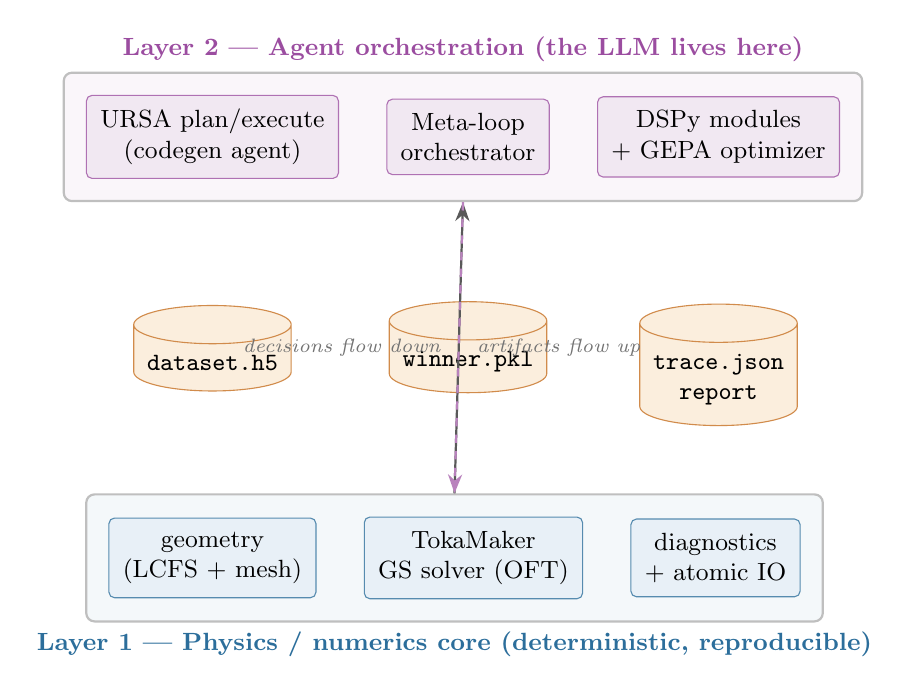
\begin{tikzpicture}[node distance=6mm]
  % Layer 2 (agent) top
  \node[agproc] (ursa)  {URSA plan/execute\\(codegen agent)};
  \node[agproc, right=of ursa] (meta) {Meta-loop\\orchestrator};
  \node[agproc, right=of meta] (dspy) {DSPy modules\\+ GEPA optimizer};
  \begin{scope}[on background layer]
    \node[lyr, fill=agent!5, fit=(ursa)(meta)(dspy),
          label={[font=\small\bfseries,text=agent]above:Layer 2 --- Agent orchestration (the LLM lives here)}] (L2) {};
  \end{scope}

  % artifacts middle
  \node[artifact, below=16mm of ursa] (dset) {dataset.h5};
  \node[artifact, below=16mm of meta] (winner) {winner.pkl};
  \node[artifact, below=16mm of dspy] (trace) {trace.json\\report};

  % Layer 1 (physics) bottom
  \node[proc, below=16mm of dset] (geom) {geometry\\(LCFS + mesh)};
  \node[proc, right=of geom] (solver) {TokaMaker\\GS solver (OFT)};
  \node[proc, right=of solver] (diag) {diagnostics\\+ atomic IO};
  \begin{scope}[on background layer]
    \node[lyr, fill=phys!5, fit=(geom)(solver)(diag),
          label={[font=\small\bfseries,text=phys]below:Layer 1 --- Physics / numerics core (deterministic, reproducible)}] (L1) {};
  \end{scope}

  % arrows
  \draw[flow] (L1.north) -- (L2.south) node[lbl,midway,right=1mm]{artifacts flow up};
  \draw[flowback] (L2.south) -- (L1.north) node[lbl,midway,left=1mm]{decisions flow down};
\end{tikzpicture}
\caption{The two-layer architecture. The language model makes only high-level decisions in
Layer~2; all numerics are deterministic Layer~1 library code. The layers exchange only on-disk
artifacts, which keeps the science reproducible and the solver's process-singleton constraint
isolated.}
\label{fig:arch}
\end{figure}

\subsection{Three phases}
The learning pipeline runs in three phases, which the outer agent may revisit in any order
(Figure~\ref{fig:phases}). Phases~1--2 are the classic ``generate data, then fit a model'' loop.
Phase~3 is the contribution that closes the loop: it \emph{measures where the current surrogate is
weak} and directs new expensive solves at exactly those regions, and it hands the high-level
``what should we do next?'' decision to an LLM.

\begin{figure}[h]
\centering
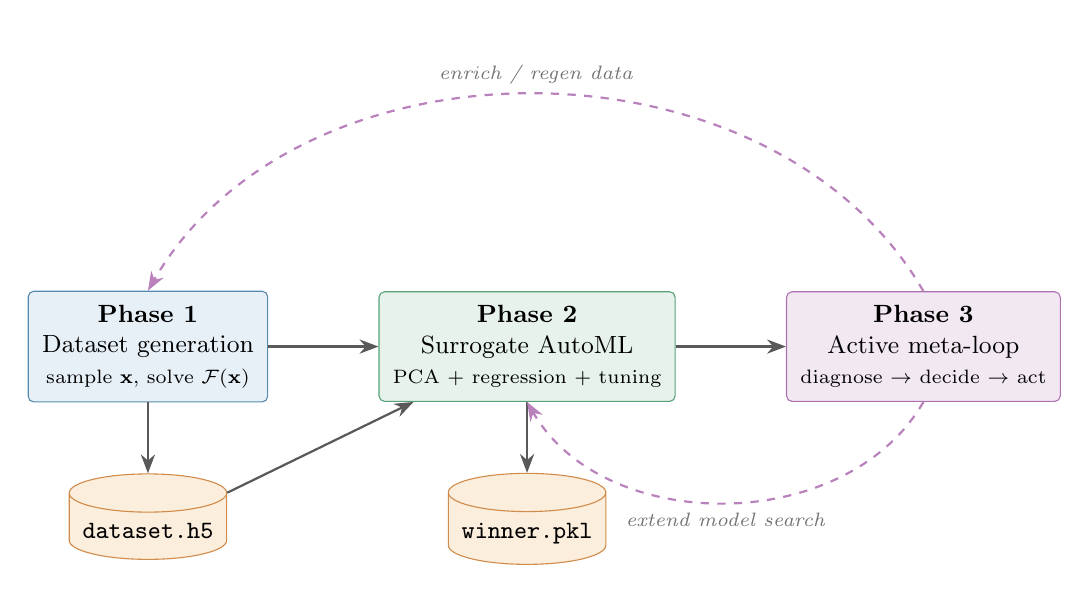
\begin{tikzpicture}[node distance=10mm]
  \node[proc]  (p1) {\textbf{Phase 1}\\Dataset generation\\{\scriptsize sample $\bx$, solve $\Ffwd(\bx)$}};
  \node[mlproc, right=14mm of p1] (p2) {\textbf{Phase 2}\\Surrogate AutoML\\{\scriptsize PCA + regression + tuning}};
  \node[agproc, right=14mm of p2] (p3) {\textbf{Phase 3}\\Active meta-loop\\{\scriptsize diagnose $\to$ decide $\to$ act}};

  \node[artifact, below=9mm of p1] (a1) {dataset.h5};
  \node[artifact, below=9mm of p2] (a2) {winner.pkl};

  \draw[flow] (p1)--(p2);
  \draw[flow] (p2)--(p3);
  \draw[flow] (p1)--(a1);
  \draw[flow] (p2)--(a2);
  \draw[flow] (a1) -- (p2);

  % feedback from meta-loop
  \draw[flowback] (p3.north) to[out=120,in=60] node[lbl,above]{enrich / regen data} (p1.north);
  \draw[flowback] (p3.south) to[out=240,in=300] node[lbl,below]{extend model search} (p2.south);
\end{tikzpicture}
\caption{The three phases and the feedback the meta-loop adds. Solid arrows are the forward
pipeline; dashed arrows are the Phase-3 decisions that send the loop back to acquire better data
(Phase 1) or search a better model (Phase 2).}
\label{fig:phases}
\end{figure}

\subsection{Notation}
\begin{center}
\begin{tabular}{@{}ll@{}}
\toprule
Symbol & Meaning \\
\midrule
$\bx=(R_0, a, \kappa, \delta, I_p)\in\R^5$ & tokamak shaping/current parameters (input) \\
$\psi(R,Z)$ & poloidal flux field (output), discretized to $\Psi\in\R^{n_Z\times n_R}$ \\
$\Ffwd$ & the true GS forward operator (TokaMaker) \\
$\Fhat$ & the learned surrogate \\
$P=n_Z\,n_R$ & number of output pixels ($96\times 64=6144$ in the shipped grid) \\
$k$ & number of retained PCA components \\
$\mathcal{D}=\{(\bx_i,\Psi_i)\}_{i=1}^N$ & dataset of solved equilibria \\
\bottomrule
\end{tabular}
\end{center}

% =====================================================================
\section{The physics forward problem}

\subsection{What we are computing, and why it is expensive}
The object of interest is the \textbf{poloidal flux} $\psi(R,Z)$, a scalar field on a 2-D slice
through the torus. Its contour lines are the magnetic surfaces on which the plasma sits, so $\psi$
\emph{is} the equilibrium: from it one derives the plasma boundary, the safety factor, the
location of the magnetic axis, and every stability metric an engineer cares about. Computing
$\psi$ means solving a nonlinear elliptic PDE on a finite-element mesh, iterating until the plasma
current and the magnetic field it produces are self-consistent. That self-consistency iteration is
what makes each solve expensive --- and what makes a learned surrogate worthwhile.

\subsection{The Grad--Shafranov equation}
TokaMaker solves the axisymmetric ideal-MHD force-balance equation --- the \textbf{Grad--Shafranov
equation} --- for $\psi(R,Z)$ in the 2-D poloidal $(R,Z)$ plane:
\begin{equation}
\Lstar\,\psi \;=\; -\,\mu_0\, R^2\, p'(\psi) \;-\; F(\psi)\,F'(\psi).
\end{equation}
Reading the equation term by term: the left-hand side is a differential operator acting on the
unknown field $\psi$; the right-hand side is the \emph{source} that the plasma's own pressure and
current supply. The two sources are what make it nonlinear --- they depend on $\psi$, the very
thing being solved for. Concretely, $\psi(R,Z)$ is the poloidal flux function, whose level sets
$\{\psi=\text{const}\}$ are the nested magnetic flux surfaces; $\Lstar$ is the \textbf{Grad--Shafranov
operator}, a non-Laplacian elliptic operator that in cylindrical coordinates reads
\begin{equation}
\Lstar\psi \;=\; R\,\frac{\partial}{\partial R}\!\left(\frac{1}{R}\frac{\partial \psi}{\partial R}\right) + \frac{\partial^2 \psi}{\partial Z^2},
\end{equation}
the extra $1/R$ factor (relative to the ordinary Laplacian) arising from the toroidal geometry.
$p(\psi)$ is the plasma pressure profile with $p'=\mathrm{d}p/\mathrm{d}\psi$; $F(\psi)=R\,B_\phi$
is the poloidal-current function ($B_\phi$ = toroidal field) with $F'=\mathrm{d}F/\mathrm{d}\psi$;
and $\mu_0$ is the vacuum permeability. Because the right-hand side is nonlinear in $\psi$,
TokaMaker solves it by Picard/Newton iteration on a triangular finite-element mesh.

\subsection{Boundary: the Last Closed Flux Surface}
An elliptic PDE needs a boundary condition. In \textbf{fixed-boundary} mode (this platform's
default) we prescribe the outermost closed contour --- the \textbf{Last Closed Flux Surface
(LCFS)} --- and solve for $\psi$ inside it. The LCFS is an analytic D-shaped curve; a standard
tokamak parameterization is
\begin{equation}
\begin{aligned}
R(\theta) &= R_0 + a\cos\!\big(\theta + \delta\sin\theta\big),\\
Z(\theta) &= Z_0 + \kappa\, a\sin\theta, \qquad \theta\in[0,2\pi),
\end{aligned}
\end{equation}
with $R_0$ the major radius of the plasma center (m), $a$ the minor radius / half-width (m),
$\kappa$ the elongation ($1=$ circular, $\approx1.6$ ITER-like), $\delta$ the triangularity
($0=$ symmetric, $>0=$ D-shaped), and $Z_0$ the vertical center (fixed to $0$ here). These are
four of our five input knobs; the fifth, the plasma current $I_p$, sets the overall magnitude of
$\psi$.

An \textbf{isoflux} constraint additionally pins $\psi$ to a constant along the sampled boundary
points, $\psi(R(\theta_j),Z(\theta_j))=\psi_b\ \forall j$. It is more accurate but numerically
fragile: on extreme shapes it can fail at construction, in which case the solver drops the
constraint and re-solves unconstrained. Whether isoflux held is recorded per sample --- an
important bookkeeping detail, because \emph{if it fell back, the geometry inputs no longer describe
the saved $\psi$} and that sample must be flagged and excluded from clean training.

\subsection{The forward operator and its feasible set}
For the learning problem we hide all of that machinery behind a single deterministic forward
operator
\begin{equation}
\Ffwd:\ \bx=(R_0,a,\kappa,\delta,I_p)\ \longmapsto\ \psi(R,Z).
\end{equation}
The output is interpolated from the FEM mesh onto a fixed rectangular grid
$\Psi\in\R^{n_Z\times n_R}$ so downstream ML can treat it as an image tensor
(Figure~\ref{fig:surrogate} makes this concrete). Pixels \emph{outside the LCFS} carry no plasma
and are set to $\mathrm{NaN}$; all metrics mask them out.

A subtlety that shapes the whole active-learning design: not every $\bx$ produces a valid solve.
Extreme shaping (high $\kappa$, high $\delta$, small $a$) drives the solver into isoflux fallback
or outright failure. We therefore treat the solver as a \emph{constrained} black box with an
unknown \textbf{feasible set}
\begin{equation}
\Omega=\{\bx: \Ffwd(\bx)\ \text{succeeds}\}\subseteq\mathcal{X},
\end{equation}
and later learn a probabilistic model of $\Omega$ (Section~\ref{sec:feas}) so we do not waste
budget solving points that will fail. The shipped seed box is $R_0\in[0.35,0.55]$~m,
$a\in[0.10,0.20]$~m, $\kappa\in[1.0,1.6]$, $\delta\in[0,0.4]$, $I_p\in[80,200]$~kA.

% =====================================================================
\section{Phase 1 --- Dataset generation}

\subsection{Choosing where to sample}
A supervised model needs examples, and each example here is one expensive solve. With a fixed
budget of $N$ solves, \emph{where} in the 5-D box we place them matters. Blind sampling uses a
space-filling design --- either \textbf{Latin Hypercube Sampling (LHS)} or a \textbf{Sobol}
low-discrepancy sequence --- rather than independent uniform draws. The reason is coverage: for a
fixed $N$, these designs spread points across the box far more evenly (they have lower
star-discrepancy), so no region is left accidentally empty and none is wastefully clustered. Every
draw is seeded, so a dataset can be regenerated bit-for-bit. Phase~3 will later replace this
``blind'' placement with a \emph{targeted} one, but blind space-filling is the right way to seed.

\subsection{The dataset tensor}
The HDF5 artifact stores, for $N$ samples: \texttt{inputs}$\in\R^{N\times 5}$ (columns
$(R_0,a,\kappa,\delta,I_p)$); \texttt{psi}$\in\R^{N\times n_Z\times n_R}$ (fields, NaN outside the
LCFS); \texttt{R},\texttt{Z} (grid axes); \texttt{success}$\in\{0,1\}^N$ (whether the isoflux
solve succeeded --- this is our labelled data for the feasibility model); and provenance for
reproducibility. One design decision is worth stating because it drives a downstream parameter:
the stored $\psi$ is \textbf{physical poloidal flux in Webers}, not per-sample normalized
$\psi_N\in[0,1]$. Normalizing each field to $[0,1]$ would erase the $I_p$ dependence entirely
(the current only sets the field's scale), which is information the surrogate must predict. Keeping
physical units means the data is \emph{less} low-rank (Section~\ref{sec:pca}), so we retain more
principal components than a normalized dataset would need.

% =====================================================================
\section{Phase 2 --- The surrogate model}

\subsection{The idea: don't predict 6144 pixels directly}
We want a cheap map $\Fhat_\theta$ that reproduces the solver's field, formally minimizing expected
field error over the input distribution $p(\bx)$:
\begin{equation}
\theta^\star=\argmin_\theta\ \E_{\bx\sim p}\Big[\ \big\|\,\Ffwd(\bx)-\Fhat_\theta(\bx)\,\big\|^2_{\text{masked}}\ \Big],
\end{equation}
where $\|\cdot\|_{\text{masked}}$ is the RMS over in-LCFS pixels and, with only the finite sample
$\mathcal{D}$, we minimize a cross-validated estimate of this loss. The output is a
$96\times64=6144$-pixel image, and regressing 6144 correlated targets directly from five inputs is
both wasteful and noisy. The key observation is that equilibrium flux fields are extremely
redundant: across a whole dataset they nearly live on a low-dimensional linear subspace. So the
surrogate \textbf{factors into two steps} (Figure~\ref{fig:surrogate}): compress the field to a
few numbers with PCA, then regress those few numbers from the five inputs.

\begin{figure}[h]
\centering
\resizebox{\textwidth}{!}{%
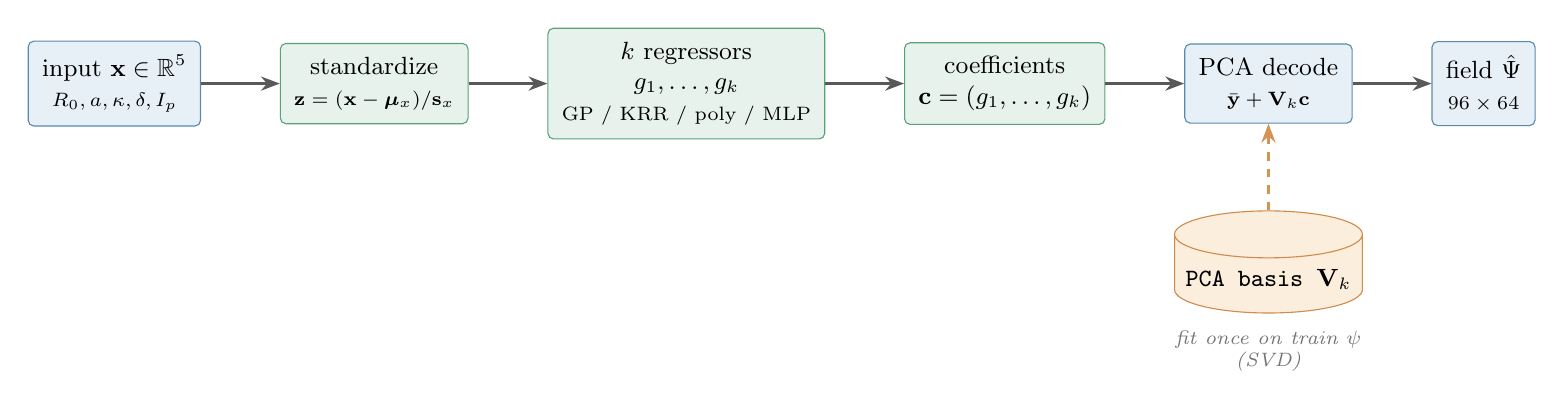
\begin{tikzpicture}[node distance=8mm]
  \node[proc] (x) {input $\bx\in\R^5$\\{\scriptsize $R_0,a,\kappa,\delta,I_p$}};
  \node[mlproc, right=10mm of x] (std) {standardize\\{\scriptsize $\bz=(\bx-\bmu_x)/\mathbf{s}_x$}};
  \node[mlproc, right=10mm of std] (reg) {$k$ regressors\\$g_1,\dots,g_k$\\{\scriptsize GP / KRR / poly / MLP}};
  \node[mlproc, right=10mm of reg] (coef) {coefficients\\$\bc=(g_1,\dots,g_k)$};
  \node[proc, right=10mm of coef] (dec) {PCA decode\\{\scriptsize $\bar\by+\bV_k\bc$}};
  \node[proc, right=10mm of dec] (psi) {field $\hat\Psi$\\{\scriptsize $96\times64$}};

  \draw[flow] (x)--(std); \draw[flow] (std)--(reg); \draw[flow] (reg)--(coef);
  \draw[flow] (coef)--(dec); \draw[flow] (dec)--(psi);

  % training-time PCA fit annotation
  \node[artifact, below=11mm of dec] (basis) {PCA basis $\bV_k$};
  \draw[flow, dashed, draw=data!80] (basis) -- (dec);
  \node[lbl, below=1mm of basis, align=center] {fit once on train $\psi$\\(SVD)};
\end{tikzpicture}%
}
\caption{The surrogate factorization. Rather than predict 6144 pixels directly, PCA compresses the
flux field to $k$ coefficients (learned once from the training fields by SVD); $k$ small regressors
map the five standardized inputs to those coefficients; and the orthonormal PCA basis $\bV_k$
decodes them back to a full field.}
\label{fig:surrogate}
\end{figure}

\subsection{Output reduction: Principal Component Analysis}
\label{sec:pca}
Flatten each field to $\by_i\in\R^P$ (NaN pixels imputed by the per-pixel training mean
$\bar\by$), stack the centered fields into $\mathbf{Y}_c=[\by_1-\bar\by,\dots]^\top\in\R^{N\times P}$,
and take its singular value decomposition
\begin{equation}
\mathbf{Y}_c = \bU\,\bSig\,\bV^\top .
\end{equation}
The first $k$ right-singular vectors $\bV_k=[\mathbf{v}_1,\dots,\mathbf{v}_k]\in\R^{P\times k}$
form an orthonormal basis ($\bV_k^\top\bV_k=\bI_k$) of the retained flux subspace --- think of each
$\mathbf{v}_j$ as an ``eigen-equilibrium'', a characteristic flux pattern, and of any field as a
weighted sum of a handful of them. Encoding and reconstruction are simply projections onto and out
of that basis:
\begin{equation}
\underbrace{\bc_i=\bV_k^\top(\by_i-\bar\by)}_{\text{encode } (P\to k)}
\qquad\qquad
\underbrace{\hat\by_i=\bar\by+\bV_k\,\bc_i}_{\text{decode } (k\to P)} .
\end{equation}
How many components we keep is governed by how much field variance each explains:
\begin{equation}
\text{EVR}_j=\frac{\sigma_j^2}{\sum_{l}\sigma_l^2},\qquad
\text{cumulative EV}(k)=\sum_{j=1}^{k}\text{EVR}_j,
\end{equation}
and $k$ is chosen (or searched) to reach a target cumulative explained variance. Because we keep
physical $\psi$ (Section~4.2), the data is \emph{less} low-rank than normalized data: $\approx 8$
components reach $\sim85\%$ EV, versus $\sim99\%$ for normalized data --- so $k$ (and the
acquisition PCA size) is set accordingly.

\subsection{Latent-space regression: the model zoo}
With the field reduced to $k$ coefficients, the learning task is $k$ ordinary scalar regressions,
$g_j:\R^5\to\R$, one per coefficient. Assembling them and decoding gives the full surrogate:
\begin{equation}
\boxed{\ \Fhat(\bx) \;=\; \bar\by \;+\; \sum_{j=1}^{k} g_j(\bx)\,\mathbf{v}_j \ }
\end{equation}
reshaped to the $n_Z\times n_R$ grid. Inputs are \emph{always} standardized first,
$\bz=(\bx-\bmu_x)/\mathbf{s}_x$, for a concrete reason: the raw features span wildly different
scales ($I_p\sim10^5$ versus $R_0\sim0.4$), so without standardization every kernel distance is
dominated by $I_p$ alone and the model collapses to predicting the mean. Four regression families
(``the zoo'') compete for each dataset; the agent chooses among them.

\paragraph{(a) Gaussian Process (GP) regression --- the headline model.} A GP is the natural
choice here because it is data-efficient at small $N$ \emph{and} returns a calibrated uncertainty
that the active-learning stage will reuse. It uses a squared-exponential (RBF) kernel plus a
white-noise term,
\begin{equation}
k(\bz,\bz') \;=\; \sigma_f^2\,\exp\!\left(-\frac{\|\bz-\bz'\|^2}{2\ell^2}\right) \;+\; \sigma_n^2\,\delta_{\bz\bz'} ,
\end{equation}
which encodes the belief that nearby inputs give similar outputs, with $\ell$ setting ``how near''.
Placing a Gaussian prior over functions and conditioning on the training data
$(\mathbf{Z},\bc^{(j)})$ yields a Gaussian \textbf{posterior predictive} at a new $\bz_\star$ with
closed-form mean and variance:
\begin{align}
g_j(\bz_\star) \;=\; \mu_j(\bz_\star) &= \mathbf{k}_\star^\top\,(\bK+\alpha\bI)^{-1}\,\bc^{(j)},\\[2pt]
\sigma_j^2(\bz_\star) &= k(\bz_\star,\bz_\star) - \mathbf{k}_\star^\top\,(\bK+\alpha\bI)^{-1}\,\mathbf{k}_\star,
\end{align}
where $\bK_{ab}=k(\bz_a,\bz_b)$ is the Gram matrix over training inputs, $\mathbf{k}_\star$ collects
the covariances between $\bz_\star$ and the training points, and $\alpha$ is a jitter/regularizer.
The prediction is a \emph{data-weighted average of observed coefficients}; the variance grows away
from the data --- which is exactly the ``I am unsure here'' signal we later exploit. The kernel
hyperparameters $(\sigma_f,\ell,\sigma_n)$ are fit by maximizing the \textbf{log marginal
likelihood}
\begin{equation}
\log p(\bc^{(j)}\mid\mathbf{Z}) = -\tfrac{1}{2}\,\bc^{(j)\top}\bK_y^{-1}\bc^{(j)} - \tfrac{1}{2}\log|\bK_y| - \tfrac{N}{2}\log 2\pi,
\quad \bK_y=\bK+\sigma_n^2\bI,
\end{equation}
which trades data fit (first term) against model complexity (second term) automatically.

\paragraph{(b) Kernel Ridge Regression (KRR).} Same kernel intuition, no uncertainty, cheaper to
fit --- useful when the GP's likelihood optimization is unstable at tiny $N$:
\begin{equation}
g_j(\bz_\star)=\mathbf{k}_\star^\top\bm{\eta},\qquad
\bm{\eta}=(\bK+\lambda\bI)^{-1}\bc^{(j)},
\end{equation}
with kernel $\in\{\text{RBF},\text{Laplacian}\}$, regularizer $\lambda$ (\texttt{alpha}), bandwidth
\texttt{gamma}.

\paragraph{(c) Polynomial ridge.} An explicit polynomial feature map $\bphi(\bz)$ of degree
$d\in\{1,2,3\}$ into ridge regression --- interpretable and fast, with a low-frequency bias that
suits smooth fields:
\begin{equation}
\bw_j=\argmin_{\bw}\ \|\bPhi\bw-\bc^{(j)}\|^2+\lambda\|\bw\|^2
=(\bPhi^\top\bPhi+\lambda\bI)^{-1}\bPhi^\top\bc^{(j)},
\qquad g_j(\bz_\star)=\bphi(\bz_\star)^\top\bw_j .
\end{equation}

\paragraph{(d) Small MLP.} A capped multilayer perceptron ($\le 2$ hidden layers, width
$\le 256$) --- a universal approximator kept small to avoid overfitting the modest dataset,
trained with L2 penalty $\alpha$ and a chosen learning rate. Deep operator/PINN/FNO families are
explicitly out of the proof-of-concept scope, so the zoo is intentionally classical and
CPU-cheap.

\subsection{AutoML: automatically tuning each model}
\label{sec:automl}
Each model has knobs (a length scale, a regularizer, a network width) whose best values are not
known in advance, so they are \emph{searched}. The objective is the honest one --- \textbf{$K$-fold
cross-validated field RMSE in physical $\psi$ units}, with the PCA refit inside each fold to avoid
leaking test information into the basis:
\begin{equation}
\mathcal{L}(\mathbf{h}) = \frac{1}{K}\sum_{f=1}^{K}
\RMSE\!\Big(\Psi_{\text{va}_f},\ \Fhat_{\mathbf{h}}^{(\text{tr}_f)}(\mathbf{X}_{\text{va}_f})\Big),
\quad
\RMSE(\Psi,\hat\Psi)=\sqrt{\frac{1}{|\mathcal{M}|}\sum_{(i,p)\in\mathcal{M}}(\Psi_{ip}-\hat\Psi_{ip})^2},
\end{equation}
where $\mathcal{M}$ is the set of finite (in-LCFS) cells. The search itself solves
\begin{equation}
\mathbf{h}^\star=\argmin_{\mathbf{h}\in\mathcal{H}}\ \mathcal{L}(\mathbf{h})
\end{equation}
using \textbf{Optuna's Tree-structured Parzen Estimator (TPE)} --- a Bayesian-optimization sampler
that, instead of a grid, learns from past trials which regions of $\mathcal{H}$ produce good
scores. It models the density of hyperparameters among the good trials, $\ell(\mathbf{h})$, and
among the poor ones, $g(\mathbf{h})$, and proposes points maximizing the ratio
$\ell(\mathbf{h})/g(\mathbf{h})$ (an expected-improvement surrogate over the \emph{configuration}
space, distinct from the GP surrogate over the \emph{physics}). A trial that crashes returns a
large sentinel objective ($10^{10}$) so the search simply moves on. When the search ends, the best
$(\text{model},\mathbf{h}^\star,k)$ is \textbf{refit on all non-test samples} and saved as
\texttt{winner.pkl} with its PCA handle.

\subsection{Did it actually learn anything? Scoring against a baseline}
A low RMSE means little on its own --- a field with small magnitude has small errors trivially. We
therefore always compare against the \textbf{trivial baseline}: predict every field as the
per-pixel mean of the training fields, $\hat\Psi^{\text{base}}=\bar\Psi_{\text{train}}$. The two
headline numbers are relative to that baseline:
\begin{equation}
\text{RMSE ratio}=\frac{\RMSE(\Fhat)}{\RMSE(\hat\Psi^{\text{base}})},
\qquad
\text{error reduction}=100\big(1-\text{RMSE ratio}\big)\ \%,
\end{equation}
so ``90\% accuracy'' means the surrogate cuts the baseline field error by 90\%, and any acceptable
winner must have RMSE ratio $<1$ (i.e.\ beat doing nothing). Additional diagnostics --- MAE,
relative $L_2$, $R^2$, correlation, tolerance-band accuracy --- are reported for interpretation.

% =====================================================================
\section{Phase 3 --- Active learning: sampling where the model is weak}

\subsection{Why blind sampling wastes budget}
Blind LHS spends the same effort everywhere, but a surrogate is rarely uniformly bad --- it is
usually accurate in the well-sampled middle of the box and poor in some corner (say, high
elongation). If our next batch of expensive solves is scattered blindly, most of it lands where the
model is \emph{already} good and teaches it little. Active learning fixes this: it uses the current
model's own errors to decide where the next solves should go, so the budget is spent closing the
weak regions. Figure~\ref{fig:active} shows the loop; the default strategy is \textbf{residual-driven
Upper Confidence Bound (residual-UCB)}, with graceful fallbacks when a trustworthy winner does not
yet exist.

\begin{figure}[h]
\centering
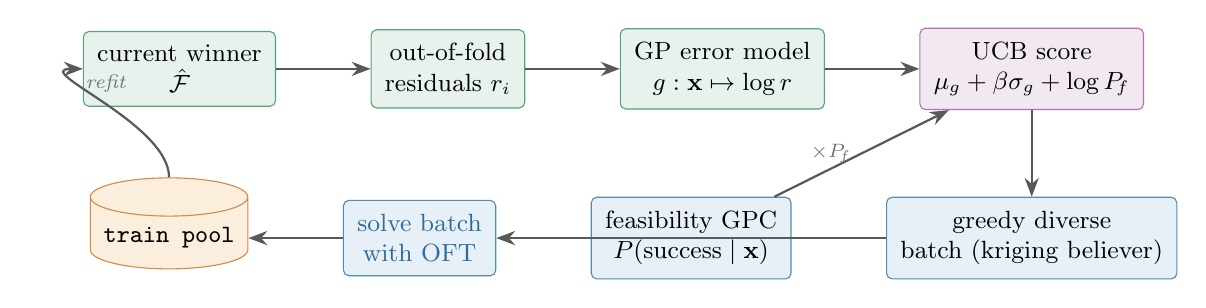
\begin{tikzpicture}[node distance=9mm]
  \node[mlproc] (winner) {current winner\\$\Fhat$};
  \node[mlproc, right=12mm of winner] (oof) {out-of-fold\\residuals $r_i$};
  \node[mlproc, right=12mm of oof] (gp) {GP error model\\$g:\bx\mapsto\log r$};
  \node[agproc, right=12mm of gp] (ucb) {UCB score\\$\mu_g+\beta\sigma_g+\log P_{\!f}$};
  \node[proc, below=11mm of ucb] (batch) {greedy diverse\\batch (kriging believer)};
  \node[proc, left=12mm of batch] (feas) {feasibility GPC\\$P(\text{success}\mid\bx)$};
  \node[phys, proc, left=12mm of feas] (solve) {solve batch\\with OFT};
  \node[artifact, left=12mm of solve] (pool) {train pool};

  \draw[flow] (winner)--(oof); \draw[flow] (oof)--(gp); \draw[flow] (gp)--(ucb);
  \draw[flow] (ucb)--(batch);
  \draw[flow] (feas)--(ucb) node[lbl,midway,left]{$\times P_{\!f}$};
  \draw[flow] (batch)--(solve);
  \draw[flow] (solve)--(pool);
  \draw[flow] (pool) to[out=90,in=180] node[lbl,above]{refit} (winner.west);
\end{tikzpicture}
\caption{The residual-driven active-learning loop. The winner's out-of-fold residuals train a GP
\emph{error model}; a UCB acquisition (discounted by a feasibility classifier) ranks a candidate
pool; a greedy ``kriging-believer'' rule picks a spread-out batch; those points are solved,
merged into the pool, and the winner is refit --- closing the loop.}
\label{fig:active}
\end{figure}

\subsection{The acquisition signal: out-of-fold residuals}
To target weakness we must first \emph{measure} it honestly. The signal is the winner's
\textbf{out-of-fold (OOF) residual} on the training pool: for each cross-validation fold we refit
the winner's architecture on the fold's training rows and record each held-out sample's mean
absolute field error,
\begin{equation}
r_i \;=\; \frac{1}{|\mathcal{M}_i|}\sum_{p\in\mathcal{M}_i}\big|\,\Psi_{ip}-\Fhat^{(-\text{fold}(i))}(\bx_i)_p\,\big| .
\end{equation}
Using OOF (not training-set) residuals is essential: interpolating models such as GP and KRR fit
their own training points to $\approx0$ error, so training residuals would report ``perfect
everywhere'' and carry no signal about \emph{generalization}. The OOF residual, by contrast,
measures error at points the fitted model has never seen --- exactly the quantity we want to reduce.

\subsection{The error model and the UCB score}
We then fit a \emph{second} GP --- the \textbf{error model} --- to predict how large the residual
will be at any candidate geometry, working with log residuals over standardized inputs,
\begin{equation}
g:\ \bx\ \longmapsto\ \log r,\qquad g\sim\GP\big(\mu_g,\,k_{\text{ARD}}\big),
\end{equation}
using an \textbf{ARD (Automatic Relevance Determination) RBF kernel} with a separate length scale
per input dimension,
\begin{equation}
k_{\text{ARD}}(\bz,\bz')=\sigma_f^2\exp\!\left(-\tfrac{1}{2}\sum_{d=1}^{5}\frac{(z_d-z'_d)^2}{\ell_d^2}\right)+\sigma_n^2\delta .
\end{equation}
Per-dimension length scales let the error model discover that weakness aligns with a few input
directions (e.g.\ elongation) and ignore the irrelevant ones. The log transform reflects that
error is multiplicatively structured and keeps a few catastrophic samples from dominating the fit.
Like any GP, this one gives a posterior mean $\mu_g(\bx)$ (predicted error) and standard deviation
$\sigma_g(\bx)$ (confidence in that prediction).

Now comes the central decision rule. We do not simply solve wherever predicted error is highest ---
that would ignore regions the error model has never seen. Instead we rank candidates by an
\textbf{Upper Confidence Bound}, written in log space so the feasibility term adds in cleanly:
\begin{equation}
\boxed{\ a(\bx) \;=\; \underbrace{\mu_g(\bx)}_{\text{exploit measured weakness}} \;+\; \beta\,\underbrace{\sigma_g(\bx)}_{\text{explore the unknown}} \;+\; \underbrace{\log P_{\text{feas}}(\bx)}_{\text{avoid infeasible solves}}\ }
\end{equation}
The first term \emph{exploits}: go where we have measured the model to be bad. The second term
\emph{explores}: go where the error model itself is uncertain --- which naturally includes regions
with no data yet, such as a target envelope wider than the seed box. The weight $\beta\in[0,3]$,
exposed to the meta-agent, tunes the balance (Figure~\ref{fig:ucb}): $\beta=0$ is pure
exploitation and may pile onto one weak pocket; larger $\beta$ pushes toward coverage. The third
term discounts candidates likely to fail. Candidates are drawn from a large Sobol pool over the
envelope bounds.

\begin{figure}[h]
\centering
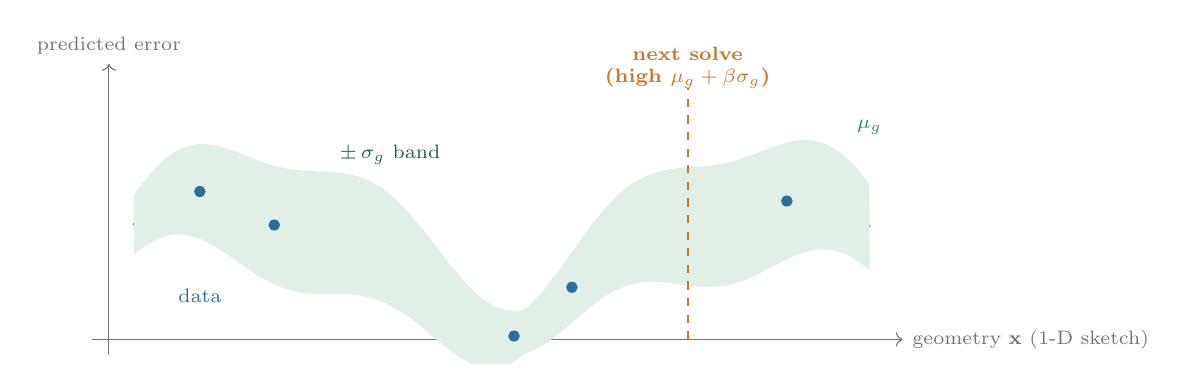
\begin{tikzpicture}[xscale=1.05,yscale=1.0]
  % axes
  \draw[->,black!55] (-0.2,0) -- (9.6,0) node[right,font=\scriptsize]{geometry $\bx$ (1-D sketch)};
  \draw[->,black!55] (0,-0.2) -- (0,3.5) node[above,font=\scriptsize]{predicted error};
  % mean curve mu_g
  \draw[ml,very thick,domain=0.3:9.2,samples=120,smooth,variable=\t]
      plot ({\t},{1.05 + 0.75*sin(\t r) + 0.28*sin(2.3*\t r)});
  % uncertainty band (sigma) -- widen away from "data" points near x=2,5,8
  \begin{scope}
  \clip (0.3,-0.3) rectangle (9.2,3.6);
  \fill[ml!14]
    plot[domain=0.3:9.2,samples=120,smooth,variable=\t] ({\t},{1.05 + 0.75*sin(\t r) + 0.28*sin(2.3*\t r) + (0.28+0.5*abs(sin(0.62*\t r +1)))})
    -- plot[domain=9.2:0.3,samples=120,smooth,variable=\t] ({\t},{1.05 + 0.75*sin(\t r) + 0.28*sin(2.3*\t r) - (0.28+0.5*abs(sin(0.62*\t r +1)))})
    -- cycle;
  \end{scope}
  % data points (small N, where sigma is small)
  \foreach \x in {1.1,2.0,4.9,5.6,8.2} {
    \fill[phys] (\x,{1.05 + 0.75*sin(\x r) + 0.28*sin(2.3*\x r)}) circle (2pt);
  }
  % acquisition pick: high mean + high sigma region (around x ~ 7)
  \draw[data,thick,dashed] (7.0,0) -- (7.0,3.2);
  \node[data,font=\scriptsize\bfseries,align=center] at (7.0,3.45) {next solve\\(high $\mu_g+\beta\sigma_g$)};
  \node[ml,font=\scriptsize] at (9.2,2.7) {$\mu_g$};
  \node[ml!70!black,font=\scriptsize] at (3.4,2.35) {$\pm\,\sigma_g$ band};
  \node[phys,font=\scriptsize] at (1.1,0.55) {data};
\end{tikzpicture}
\caption{The exploit/explore intuition behind the UCB (schematic, 1-D). The green curve is the
error model's predicted error $\mu_g$; the band is its uncertainty $\pm\sigma_g$, which widens away
from the sampled points (blue). The acquisition prefers points that are both predicted-bad
\emph{and} uncertain, so the next solve lands where the model is most likely weak yet under-explored
--- not merely at the tallest known peak.}
\label{fig:ucb}
\end{figure}

\subsection{Feasibility weighting: modeling the feasible set $\Omega$}
\label{sec:feas}
A failed solve costs the same wall-clock as a successful one, so it is worth learning which
geometries fail. A GP classifier (GPC) with an ARD-RBF kernel is trained on \emph{every attempted
input}, successes and failures alike (this is why Phase~1 records the \texttt{success} flag),
giving $P(\text{success}\mid\bx)$. The acquisition is discounted by the \emph{squared} probability,
floored:
\begin{equation}
P_{\text{feas}}(\bx) \;=\; \max\!\Big(\,P(\text{success}\mid\bx)^2,\ \varepsilon\,\Big),\qquad \varepsilon=0.02 .
\end{equation}
Squaring prevents a known-bad region from out-bidding a merely well-covered feasible one on prior
variance alone; the (deliberately harsh) floor $\varepsilon$ keeps an unlucky region down-weighted
but never permanently written off. If the GPC fails to fit, a distance-weighted $k$-NN estimate is
used instead. ARD matters here for the same reason as before: failures align with a few shaping
directions, and an isotropic distance would let the irrelevant dimensions blur that boundary.

\subsection{Batch selection: picking a spread-out batch, not one point $n$ times}
We usually want a \emph{batch} of $n$ new solves at once, and na\"ively taking the top-$n$
acquisition scores would return $n$ near-duplicates clustered on a single peak. The fix rests on a
special property of GPs: \textbf{the posterior variance depends only on \emph{where} you have
observed, not on \emph{what} you observed}. So under the ``kriging-believer'' heuristic we pretend
each pick was observed at the model's own mean --- which leaves $\mu_g$ unchanged but shrinks
$\sigma_g$ around it --- and then re-score. Concretely:
\begin{enumerate}[leftmargin=*]
  \item Pick $\bx^{(1)}=\argmax_{\bx} a(\bx)$.
  \item Condition the GP variance on $\bx^{(1)}$ (an exact rank-1 Cholesky update), lowering
  $\sigma_g$ --- and hence $a$ --- in its neighborhood.
  \item Re-score the remaining pool and repeat until $n$ points are chosen.
\end{enumerate}
Because only the variance changes, the update is exact and cheap ($O(n\cdot m)$ per pick for $m$
candidates), and the batch automatically spreads out to cover the weak \emph{region} rather than a
single weak \emph{point}.

\subsection{Fallbacks: when there is no trustworthy winner yet}
Early on --- before Phase~2 has produced a reliable winner, or when a residual fit fails
numerically --- the acquisition degrades gracefully down a ladder, and records which rung it used:
\begin{equation}
\texttt{residual\_ucb}\ \longrightarrow\ \texttt{gp\_variance}\ \longrightarrow\ \texttt{maximin\_fallback}.
\end{equation}

\paragraph{gp\_variance (the ALM criterion).} Without a winner to critique, we fall back to a
model-agnostic notion of ``where is the field itself most uncertain''. Fit one GP per PCA component
(an independent emulator) and score a candidate by the total predictive variance of the
\emph{reconstructed} field. Because the PCA basis is orthonormal, that pixel-summed variance
collapses \textbf{exactly} to a weighted sum of per-component variances --- no sampling, no
approximation:
\begin{equation}
\sum_{\text{pixels}}\Var\big[\hat\psi(\bx)\big] \;=\; \sum_{j=1}^{k} s_j^2\,\sigma_j^2(\bx),
\end{equation}
where $s_j$ is the train-set standard deviation of coefficient $j$ and $\sigma_j^2(\bx)$ is that
component's posterior variance. This is the classical Active-Learning-MacKay (ALM) criterion,
selected greedily with the same exact variance conditioning and the same feasibility weighting.

\paragraph{maximin\_fallback.} With too few successful solves to trust \emph{any} GP ($<8$), we
give up on error modeling entirely and just spread out: greedy feasibility-weighted \textbf{maximin
space-filling} in standardized input space, where each new point maximizes its (feasibility-weighted)
distance to everything attempted so far:
\begin{equation}
\bx^{(t+1)} = \argmax_{\bx\in\text{pool}}\ P_{\text{feas}}(\bx)\cdot \min_{\bx'\in\text{chosen}\,\cup\,\text{attempted}} \|\bx-\bx'\| .
\end{equation}
Even this floor is better than another blind LHS batch, because it still avoids known-infeasible
regions and never re-samples where we already have data.

\subsection{Honest evaluation: the frozen envelope and per-cell errors}
Active learning creates a measurement problem. Once we sample geometries \emph{outside} the seed
box, a test set carved from the seed dataset no longer represents the geometries we care about ---
it measures accuracy on the wrong distribution. The fix is a single \textbf{frozen, full-envelope
evaluation set}: $n_{\text{eval}}$ points (default 256) are drawn once by LHS over the \emph{target
envelope} (the seed box widened and clipped to physically sane values), solved, and never grown, so
every winner across every meta-iteration is judged on identical samples. The acquisition draws over
that same envelope, so the distribution we \emph{evaluate} on and the distribution we \emph{acquire}
in agree.

There is also a subtler point: an aggregate RMSE can hide exactly the failure active learning is
meant to fix. ``Great in the seed box, broken at high $\kappa$'' and ``uniformly mediocre'' can
share the same average. So scoring is \textbf{stratified per geometry cell}: each eval sample is
binned into a joint cell ($n_b$ bins per dimension $\Rightarrow n_b^5$ cells), plus per-parameter
tercile marginals, and RMSE is computed per occupied cell. The headline quantities are
\begin{equation}
\text{worst\_cell\_rmse}=\max_{c\in\text{occupied}}\RMSE_c,\qquad
\text{mean\_cell\_rmse}=\frac{1}{|\mathcal{C}|}\sum_{c\in\mathcal{C}}\RMSE_c,
\end{equation}
the latter weighting every geometry region equally regardless of how many samples landed in it. An
early-stopping bar can even be phrased per cell --- stop only once \emph{every} occupied cell beats
its own local baseline by the target margin, $\min_c 100\,(1-\RMSE_c/\RMSE_c^{\text{base}})\ge\tau$
--- which directly rewards fixing the weakest region.

\subsection{Proving it works: the control arm}
Active sampling should be \emph{demonstrably} better than blind sampling, not just plausibly so.
The blind-LHS action \texttt{regen\_dataset} is therefore retained unchanged as an \textbf{A/B
control}. The headline experiment fixes the seed dataset and the budgets and compares
\texttt{enrich\_active} against \texttt{regen\_dataset} on the same frozen envelope eval set, judged
on \textbf{worst-cell RMSE reduction per OFT solve spent}.

% =====================================================================
\section{The meta-loop --- outer optimization by an LLM agent}
\label{sec:meta}

\subsection{The decision problem}
Everything so far --- generate data, fit a model, actively acquire --- are \emph{actions}. The
meta-loop is what decides, at each step, which action to take. It is a sequential decision process
(Figure~\ref{fig:meta}): at iteration $t$ the system computes a deterministic \textbf{diagnosis} of
the current state (dataset statistics, winner metrics, per-cell errors, feasibility rates), the LLM
reads that diagnosis and emits one \textbf{typed action} $u_t$ from a small vocabulary, the action
is dispatched by deterministic code, and the resulting state is scored --- then the cycle repeats.
The action space is
\begin{equation}
u_t\in\mathcal{A}=\{\ \texttt{regen\_dataset},\ \texttt{enrich\_active},\ \texttt{extend\_search},\ \texttt{terminate}\ \}:
\end{equation}
\texttt{regen\_dataset(overrides)} reshapes or resamples the dataset (blind LHS --- the control
arm); \texttt{enrich\_active($n_{\text{new}}$, strategy, $\beta$)} runs the active-learning
acquisition of Section~6; \texttt{extend\_search(focus)} runs a fresh Phase-2 AutoML round with
directives (which models to emphasize, which hyperparameters to widen, the trial budget); and
\texttt{terminate(reason)} stops. Crucially the action is emitted as \emph{validated structured
JSON}, so the action space is small, typed, and checked before anything runs --- the LLM cannot
invent an unsupported action or a malformed payload. The loop halts when the agent terminates, when
an early-stopping quality bar is met (absolute RMSE, RMSE ratio, aggregate accuracy, or the strict
per-cell worst-cell accuracy), or when a max-iteration safety cap is reached.

\begin{figure}[h]
\centering
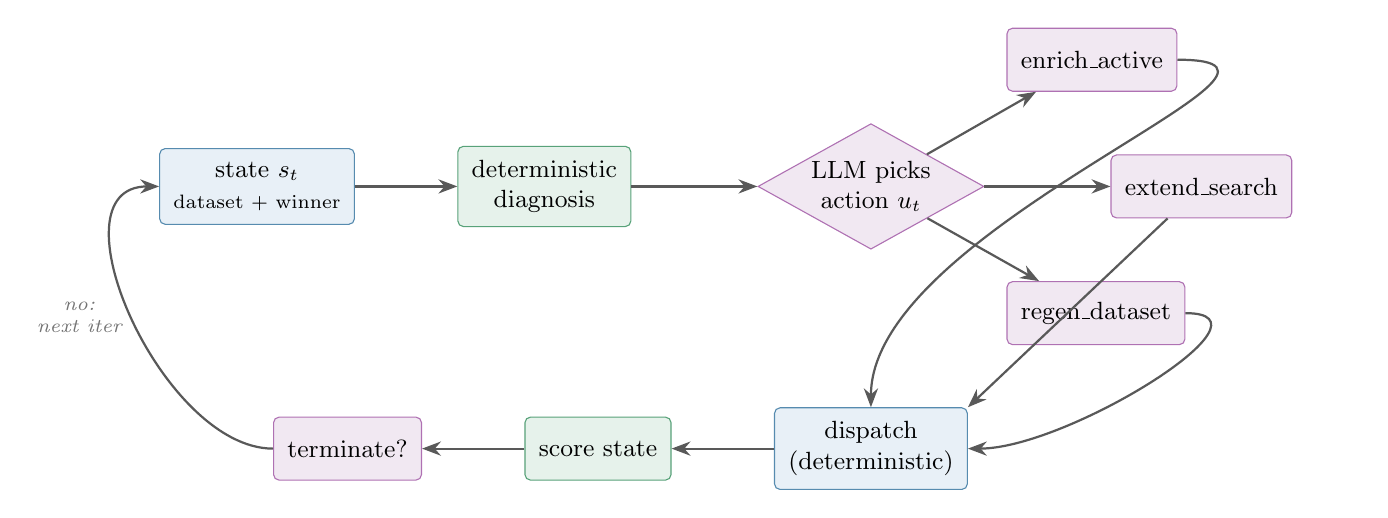
\begin{tikzpicture}[node distance=13mm]
  \node[proc] (state) {state $s_t$\\{\scriptsize dataset + winner}};
  \node[mlproc, right=of state] (diag) {deterministic\\diagnosis};
  \node[decision, right=16mm of diag] (llm) {LLM picks\\action $u_t$};
  \node[agproc, above right=8mm and 10mm of llm] (a1) {enrich\_active};
  \node[agproc, right=16mm of llm] (a2) {extend\_search};
  \node[agproc, below right=8mm and 10mm of llm] (a3) {regen\_dataset};
  \node[proc, below=20mm of llm] (disp) {dispatch\\(deterministic)};
  \node[mlproc, left=of disp] (score) {score state};
  \node[agproc, left=of score] (term) {terminate?};

  \draw[flow] (state)--(diag);
  \draw[flow] (diag)--(llm);
  \draw[flow] (llm)--(a1); \draw[flow] (llm)--(a2); \draw[flow] (llm)--(a3);
  \draw[flow] (a1) to[out=0,in=90] (disp.north);
  \draw[flow] (a2) -- (disp.north east);
  \draw[flow] (a3) to[out=0,in=0] (disp.east);
  \draw[flow] (disp)--(score);
  \draw[flow] (score)--(term);
  \draw[flow] (term) to[out=180,in=180] node[lbl,left,align=center]{no:\\next iter} (state.west);
\end{tikzpicture}
\caption{The meta-loop decision cycle. A deterministic diagnosis summarizes the state; the LLM
(the only learned component) emits a typed action; deterministic code dispatches it and re-scores;
the loop continues until the agent terminates or a quality bar / iteration cap is hit.}
\label{fig:meta}
\end{figure}

\subsection{Division of labor: what is learned vs.\ what is deterministic}
The design draws a hard line between judgment and computation, so that the science stays
reproducible while the LLM still does something genuinely open-ended:

\begin{center}
\begin{tabular}{@{}ll@{}}
\toprule
Job & Owner \\
\midrule
Which meta-action to take, and its knobs ($n_{\text{new}}$, $\beta$) & LLM (DSPy module, GEPA-optimizable) \\
Which nested Phase-2 round to run & LLM (DSPy module) \\
Acquisition core (residual GP, UCB, batch, feasibility) & Deterministic library \\
Diagnosis of current state & Deterministic library \\
Open-ended representation / data-engineering search & URSA code-generation agent \\
\bottomrule
\end{tabular}
\end{center}

Everything numerically load-bearing --- the GP kernels, the UCB arithmetic, the CV folds --- is
deterministic library code; only the \emph{high-level choices} are the LLM surface. This is what
lets the platform claim reproducible results while still being ``agentic''.

\subsection{Grading the agent: the meta-objective and GEPA}
How do we know a whole meta-run was \emph{good}, and how do we improve the agent that produced it?
Each run is graded by a composite objective that first checks correctness (\textbf{hard gates},
all of which must pass for any credit) and then rewards quality:
\begin{equation}
S \;=\;
\Big(\textstyle\prod_{g\in\text{gates}}\indic[g\ \text{passes}]\Big)
\cdot \sum_{q}\ w_q\,Q_q,
\qquad \sum_q w_q = 1 .
\end{equation}
The gates verify that the deliverables exist, the report parses, an iteration log is present, and
the winner actually loads and predicts --- a run that fails any of these scores zero, no matter how
good its numbers look. The quality terms then encode what ``good judgment'' means:

\begin{center}
\begin{tabular}{@{}llc@{}}
\toprule
Term & Meaning & $w_q$ \\
\midrule
\texttt{final\_rmse\_vs\_baseline} & $1-\RMSE_{\text{final}}/\RMSE_{\text{base}}$, clipped to $[0,1]$ & 0.35 \\
\texttt{improvement\_over\_iterations} & $(\RMSE_{\text{first}}-\RMSE_{\text{last}})/\RMSE_{\text{first}}$ & 0.20 \\
\texttt{budget\_efficiency} & fraction of total improvement by the halfway iteration & 0.10 \\
\texttt{no\_waste} & fraction of post-first-winner iterations improving RMSE $\ge1\%$ & 0.15 \\
\texttt{terminated\_by\_agent} & decisive stop (agent-chosen or target-reached) vs.\ cap-riding & 0.15 \\
\texttt{runner\_cleanliness} & only valid action types were used & 0.05 \\
\bottomrule
\end{tabular}
\end{center}

Note what these weights buy: a decisive short run that stops once it is good scores \emph{higher}
than a budget-burning run that reaches the same accuracy but keeps churning --- an explicit pressure
toward efficiency, not just accuracy. Finally, the agent itself is improved against this score. Its
decision module is written in \textbf{DSPy}, and its prompt/instructions are optimized by
\textbf{GEPA}, a reflective prompt-evolution optimizer that searches instruction variants to
maximize the expected score $\E[S]$ across recorded meta-traces. DSPy is retained \emph{only} for
this GEPA-optimizability (and as a clean way to write typed LLM programs); the numerical pipeline
does not depend on it.

% =====================================================================
\section{The agent layer (URSA) in more detail}

The two layers of Figure~\ref{fig:arch} deserve a closer look at the orchestration side.
\textbf{Layer~1 (\texttt{core})} is the stable physics/IO substrate: config schema, LCFS + mesh
construction, the TokaMaker solve with isoflux-fallback retry, diagnostic scalar extraction
($R_{\text{axis}}$, $q_0$, $q_{95}$, \dots), atomic file writes, and ordered logging. It carries one
hard invariant that shapes all parallelism: \texttt{OFT\_env} is a \textbf{process-wide singleton}
(only one per Python interpreter), so any fan-out over solves must be process-level (subprocess or
\texttt{spawn}), never threads --- a constraint the orchestration layer respects everywhere.

\textbf{Layer~2 (\texttt{agent})} is the URSA plan/execute machinery, the prompt specifications it
consumes, the meta-loop orchestrator, and the DSPy scorers/modules. It offers two runner styles.
In \emph{structured} mode the deterministic library runs the pipeline and the LLM makes one typed
decision per round --- maximally reproducible. In \emph{codegen} mode a URSA agent actually
\emph{writes} the runner script: a \texttt{PlanningAgent} emits a sequence of steps, an
\texttt{ExecutionAgent} writes code for each, runs it, inspects the output, and threads a summary
into the next step, and a feedback variant re-invokes the planner with the execution history so it
can patch failures. The agent's genuinely open-ended role is the \textbf{representation /
data-engineering search}: under a fixed evaluation protocol it reads the model diagnostics and
authors and evaluates alternative input featurizations and output transforms --- the one part of
the pipeline deliberately left to code-generating LLM search rather than to a fixed library. Every
run also writes an \texttt{experiments/<run\_id>/trace.json} and a self-contained HTML report for
inspection.

% =====================================================================
\section{Summary}

Autotokamak treats an expensive FEM equilibrium solver as a black-box forward operator
$\Ffwd:\R^5\to\psi(R,Z)$ and learns a fast surrogate $\Fhat$ by (i) reducing the flux field to a
handful of PCA coefficients, (ii) regressing each coefficient from the shaping parameters with a
small zoo of models (GP, kernel-ridge, poly-ridge, MLP), (iii) tuning hyperparameters by TPE
Bayesian optimization against cross-validated field RMSE, and (iv) actively growing the training
set with a residual-driven UCB acquisition that fits a GP error model to the winner's out-of-fold
residuals, discounts by a GP-classifier feasibility model, and selects a diverse batch by exact
kriging-believer variance conditioning. An outer meta-loop --- whose high-level decisions are made
by a DSPy/GEPA-optimized LLM and whose numerics are deterministic library code --- iterates these
phases against a frozen full-envelope, per-geometry-cell evaluation set, measuring and closing
exactly where the surrogate is weak.

The recurring mathematical objects --- the Grad--Shafranov PDE, the orthonormal PCA basis, the GP
posterior mean/variance, the cross-validated RMSE objective, the UCB acquisition, and the gated
composite meta-score --- are the load-bearing formulas of the entire system, and the diagrams above
(architecture, three-phase flow, surrogate factorization, active-learning loop, UCB intuition, and
the meta-loop cycle) are the map that ties them together.

\end{document}
